\documentclass[titlepage,parskip=half]{scrartcl}

\usepackage[margin=1in]{geometry}
\usepackage[ngerman]{babel}
\usepackage{graphicx}
\usepackage[utf8x]{inputenc}
\usepackage{csquotes}
\usepackage{tabularx}
\usepackage{enumitem}
\usepackage{lmodern,textcomp}
\usepackage{todonotes}
% \setkomafont{disposition}{\bfseries}


\title{Zusammenfassung Wirtschaft}
\author{Richard Wohlbold}

\let\Section\section
\renewcommand\section{\clearpage\Section}

\begin{document}

\maketitle
\setcounter{tocdepth}{2}
\tableofcontents
\clearpage

\section{Allgemeines}
\subsection{Definitionen}
\subsubsection{Effektivität}
Effektivität ist ein Maß für die Wirksamkeit einer Maßnahme, d.h. wie nah ein erzieltes Ergebnis dem angestrebten Ziel kommt.

\subsubsection{Effizienz}
Effizienz stellt das Verhältnis von Input zu Output sowie Leistung zu Kosten dar und beschreibt somit die Wirtschaftlichkeit einer Maßnahme.

\subsubsection{Nachhaltigkeit}
Nachhaltigkeit ist ein Handlungsprinzip zur Ressourcennutzung, bei dem eine dauerhafte Be\-dürf\-nis\-be\-frie\-di\-gung durch die Bewahrung der natürlichen Regenerationsfähigkeit der beteiligten Systeme gewährleistet werden soll.

\subsection{Arten von...}
\subsubsection{Nachhaltigkeit}
ökonomisch, ökologisch, sozial

\subsubsection{Gerechtigkeit}
Bedarfsgerechtigkeit, Verteilungsgerechtigkeit, Leistungsgerechtigkeit, Gleichheit, Generationengerechtigkeit, Gleichberechtigung

\subsection{Kriterien}
\begin{tabularx}{\textwidth}{|X|X|} \hline
    \textbf{Sachkriterien} & \textbf{Wertkriterien} \\ \hline
    Effizienz & Gerechtigkeit \\ \hline
    Effektivität & Nachhaltigkeit \\ \hline
    Legalität & Legitimität \\ \hline
    Durchsetzbarkeit & Demokratie \\ \hline
    Umsetzbarkeit & Freiheit \\  \hline
    Folgen & Gemeinwohl \\ \hline
    Stabilität & \\ \hline
    Transparenz & \\ \hline
\end{tabularx}

\section{Ökonomische Grundlagen}

\subsection{Knappheit}

\textbf{Knappheit} ist das Kernprinzip des Wirtschaftens:
\begin{itemize}
    \item Knappheit an Produkten / Gütern
    \item Knappheit an Geldmitteln / Kapital
    \item Knappheit an Zeit
\end{itemize}


\subsubsection{Was heißt knapp?}
Ein Gut ist \textbf{knapp}, wenn bei einem Preis von 0 die Nachfrage das Angebot übersteigt.


\subsubsection{Folgen der Knappheit}
\begin{itemize}
    \item Verzicht auf Entscheidungsalternativen
    \item Ungestillte Bedürfnisse, die bei Dritten durch Nutzung eines knappen Guts entstehen
    
\end{itemize}

\subsubsection{Die Maslow'sche Bedürfnispyramide}
Der amerikanische Psychologe Abraham H. Maslow entdeckte, dass unsere Bedürfnisse hierarchisch geordnet sind:\newline
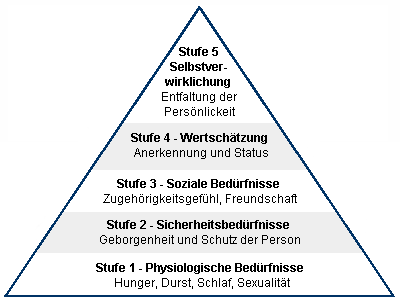
\includegraphics[width=0.5\textwidth]{bilder/maslow.png}


\subsection{Das ökonomische Prinzip}
Aufgrund der Knappheit der Güter setzen Wirtschaftssubjekte bei ihrem Handeln die eingesetzten Mittel (Kosten) mit dem Ergebnis (Nutzen) ins Verhältnis und steben eine Maximierung dieses Verhältnisses an:

$$
\textrm{Effizienz} = \frac{\textrm{Ergebnis}}{\textrm{Aufwand}} = \textrm{maximal}
$$

Dabei können diese Subjekte nach verschiedenen Formen handeln:

\subsubsection{Minimalprinzip}
Bei einem gegebenen Nutzen die Kosten minimieren.

\subsubsection{Maximalprinzip}
Bei gegebenen Kosten den Nutzen maximieren.

\subsubsection{Opportunitätskosten} 
\textbf{Opportunitätskosten} sind entgangene Erlöse, die dadurch entstehen, dass vorhandene Mög\-lich\-kei\-ten (Opportunitäten) nicht wahrgenommen wurden.


\subsection{Marginalbetrachtung}
Das \textbf{Marginalprinzip} bezeichnet ein ökonomisches Prinzip, bei dem bei jeder Mengeneinheit der neu entstandene Nutzen (\textbf{Grenznutzen}) mit den neu entstandenen Kosten (\textbf{Grenzkosten}) verglichen wird. Sollten die Grenzkosten den Grenznutzen übersteigen, so hört man auf, mehr Mengeneinheiten zu tauschen. Dies funktioniert, da mit jeder zusätzlichen Mengeneinheit der Grenznutzen dieser sinkt, die Kosten meist jedoch gleich bleiben.

Der deutsche Volkswirt Hermann Heinrich Gossen hat zwei Gesetze zum Marginalprinzip aufgestellt:

\subsubsection{1. Gossensches Gesetz}
Mit der zunehmenden Menge eines Gutes sinkt der Nutzen, den jede weitere Mengeneinheit stif\-tet.

\subsubsection{2. Gossensches Gesetz}
Ein Individuum maximiert seinen Gesamtnutzen, wenn der Nutzen der letzten ausgegebenen Geldeinheit für sämtliche Verwendungsarten gleich groß ist.


\subsection{Homo oeconomicus}

\subsubsection{Merkmale des Homo oeconomicus}
Der \textbf{Homo oeconomicus} ist ein theoretisches Modell eines ausschließlich wirtschaftlich denkenden Menschen. Er
\begin{itemize}
    \item handelt uneingeschränkt rational
    \item strebt danach, den eigenen Nutzen zu maximieren
    \item verfügt über ein widerspruchsfreies Zielsystem
    \item handelt immer zu seinem Vorteil
    \item verfügt über vollständige Information
    \item verfügt über volständige Voraussicht
\end{itemize}

\subsubsection{Probleme des Homo oeconomicus}
Richtige Menschen
\begin{itemize}
    \item maximierten nicht jederzeit seinen persönlichen Nutzen
    \item sind oft irrational
    \item achten weniger auf absolute Werte, als auf Veränderungen und überreagieren auf diese
    \item haben Abneigungen gegen Menschen, die unfair sind
\end{itemize}


\section{Der Markt}

Der Markt benutzt den Homo oeconomicus und sorgt dafür, dass alle glücklich sind:
\begin{itemize}
    \item Geschäfte werden nur abgewickelt, wenn Läufer und Verkäufer darin einen Nutzen sehen
    \item Dies funktioniert, da der Wert eines Guts immer individuell bestimmt wird.
    \item Der schottische Ökonom Adam Smith beschrieb dies durch den Ausdruck der \textbf{unsichtbare}n \textbf{Hand}. Diese bezeichnet die unbewusste Förderung des Gemeinwohls durch den Markt und die automatische Selbstregulierung zur optimalen Produktionsmenge und -qualität.
\end{itemize}

\subsection{Definitionen}
\begin{itemize}
    \item Die \textbf{Sättigungsmenge} bezeichnet die Menge an Gütern, ab der auch bei einem Preis von 0 die Nachfrage nicht weiter steigt.
    \item Der \textbf{Prohibitivpreis} bezeichnet den Preis, ab dem ein Gut nicht mehr nachgefragt wird.
    \item \textbf{Superiore Güter} sind Güter, deren Nachfrage bei steigendem Einkommen steigt.
    \item \textbf{Inferiore Güter} sind Güter, deren Nachfrage bei steigendem Einkommen sinkt.
    \item \textbf{Substitutionsgüter} sind Güter, die sich ganz oder teilweise ersetzen, ohne dass die Bedürfnisbefriedigung eingeschränkt wird.
    \item \textbf{Komplementärgüter} sind Güter, deren Konsum den Konsum anderer Güter zufolge hat.
\end{itemize}

\subsection{Funktionen des Markts}
\begin{itemize}
    \item \textbf{Informationsfunktion}: Knappheit eines Guts (Knappheitsindikator)
    \item \textbf{Koordinationsfunktion}: Planung des Angebots und der Nachfrage basierend auf dem Preis (Ausgleich von Angebot und Nachfrage)
    \item \textbf{Selektionsfunktion}: Nur Unternehmen können überleben, die kostendeckend arbeiten (Zuteilung und Auslese)
    \item \textbf{Allokationsfunktion}: Kapazizät wird dahin gelenkt, wo sie gebraucht wird (Anreize und Lenkung)
\end{itemize}

\subsection{Allmende-Problem}
Bei individualisiertem Nutzen und kollektivierten Kosten gibt es Probleme. Dies wird als das \textbf{Allmende-Problem} bezeichnet.

Beispiele: Überfischung der Meere, Umweltverschmutzung

\subsection{Eigentum}
Die Möglichkeit des Ausschlusses vom Gebrauch einer Sache ist eine Bedingung für die rationelle Nutzung knapper Ressourcen. Dies ist über das Eigentum geregelt.

Wenn eine Ressource niemandes Eigentum ist, kommt es oft zum \textbf{Allmende-Problem}.

\subsection{Wie entstehen Preise?}
\begin{itemize}
    \item Je höher der Preis für ein Gut ist, desto mehr wird von diesem Gut auf dem Markt angeboten.
    \item Je höher der Preis für ein Gut ist, desto weniger wird dieses Gut nachgefragt werden.
    \item Der Schnittpunkt der Angebots- und Nachfragekurve wird als \textbf{Gleichgewichtspreis} bezeichnet. Hier gibt es weder einen Angebots- noch einen Nachfrageüberschuss.
    \item Können Angebot und Nachfrage nicht frei spielen, so spielt sich der Gleichgewichtspreis nicht ein. Folge: Angebots- oder Nachfrageüberschüsse
\end{itemize}

\subsection{Preiselastizität}
Die \textbf{Preiselastizität} ist ein Maß dafür, wie sich die Nachfrage bei sich ändernden Preisen verändert. Sie bereichnet sich folgendermaßen:

$$
\textrm{Preiselastizität} = EL = \frac{\textrm{Änderung der Nachfrage}}{\textrm{Änderung des Preises}} = \frac{\Delta N}{\Delta P}
$$

\subsubsection{Preiselastische Nachfrage}
Eine Nachfrage mit $EL < -1$ wird als preiselastisch bezeichnet. Hier verändert sich die Nachfrage stärker als der Preis.\newline
\textit{Beispiel}: Unterhaltungselektronik, nice-to-have-Güter

\subsubsection{Preisunelastische Nachfrage}
Eine Nachfrage mit $0 > EL > -1$ wird als preisunelastisch bezeichnet. Hier verändert sich die Nachfrage weniger als der Preis.\newline
\textit{Beispiel}: Nahrungsmittel, Heizöl

\subsubsection{Vollkommen preisunelastische Nachfrage}
Eine Nachfrage mit $EL = 0$ wird als vollkommen preisunelastisch bezeichnet. Hierbei reagiert die Nachfrage gar nicht auf sich ändernde Preise.\newline
\textit{Beispiel}: Medikamente

\subsubsection{Inverse Preiselastizität (Snob-Effekt)}

Eine Nachfrage mit $EL > 0$ wird als invers preiselastisch bezeichnet (auch Snob-Effekt). Hierbei steigt die Nachfrage mit steigendem Preis.\newline
\textit{Beispiel}: Luxusgüter

\subsubsection{Einflussfaktoren}

\begin{itemize}
    \item \textbf{Substituierbarkeit}: Wenn ein Produkt nicht leicht substituiert werden kann, ist die Nachfrage tendenziell eher unelastisch.
    \item \textbf{Leichtigkeit der Nachfragebefreidigung}: Kann ein Kundenbedürfnis leicht befreidigt wird, ist die Nachfrage eher unelastisch: Große Preisreduktionen bei z.B. Salz hätten keine großen Absatzsteigerungen zufolge.
    \item \textbf{Dauerhaftigkeit}: Sind die Preise nach den Konsumenten moentan zu hoch, kann der Kauf dauerhafter Güter länger aufgeschoben werden. Somit ist die nachfrage tendenziell elastischer.
    \item \textbf{Dringlichkeit}: Eine hohe Dringlichkeit der Bedürfnisbefriedigung macht die Nachfrage weitgehend unelastisch.
\end{itemize}
    
\subsection{Der vollkommene Markt}
Der vollkommene Markt ist ein wirtschaftstheoretisches Modell. Er besitzt folgende Merkmale:
\begin{itemize}
    \item Anbieter und Nachfrager handeln nach den ökonomischen Grundprinzipien (\textit{homo oeconomicus})
    \item Das gehandelte Gut ist homogen
    \item Keine räumlichen und zeitlichen Differenzierungen
    \item Vollständige Transparenz
    \item Keine persönlichen Präferenzen unter den Marktteilnehmern
    \item Punktmarkt
\end{itemize}

\subsection{Marktformen}
Es gibt verschiedene Marktformen.

\subsubsection{Polypol}
\begin{itemize}
    \item Viele kleine Anbieter und viele kleine Nachfrager
    \item Bestmögliche Marktform der Marktwirtschaft
    \item Reger Wettbewerb 
    \item Möglichkeit, den Anbieter bei Preisänderungen zu ändern
\end{itemize}

\subsubsection{Oligopol}
\begin{itemize}
    \item Wenige Anbieter und viele kleine Nachfrager
    \item Häufig auftretende Marktform
    \item Marktmacht liegt bei wenigen Anbietern
    \item Scharfer Wettbewerb; Gefahr von Kartellbildung
\end{itemize}

\subsubsection{Monopol}
\begin{itemize}
    \item Ein Anbieter und viele kleine Nachfrager (Angebotsmonopol) oder ein Anbieter und ein Nachfrager (bilaterales Monopol)
    \item Freie Preisgestaltung durch den \textbf{Preisfixierer}, \textbf{Mengenanpasser} kann nur die abgenommende Menge Veränderungen
    \item Stellung oft nicht vollständig ausgenutzt $\Rightarrow$ Ausnutzung hätte neuen Wettbewerb zufolge 
\end{itemize}

\subsection{Wohlfahrt}
\subsubsection{Konsumentenrente}
Die Konsumentenrente berechtnet sich folgendermaßen:
$$
\textrm{Konsumentenrente} = \textrm{individuelle Zahlungsbereitschaft} - \textrm{Marktpreis}
$$

\subsubsection{Produzentenrente}
Die Produzentenrente berechtnet sich folgendermaßen:
$$
\textrm{Produzentenrente} = \textrm{Marktpreis} - \textrm{Reservationspreis}
$$
Der Reservationspreis wird auch Abgabepreis-Untergrenze genannt. 

\subsubsection{Gesamtwohlfahrt}
Die Gesamtwohlfahrt berechtnet sich folgendermaßen:
$$
\textrm{Gesamtwohlfahrt} = \textrm{Konsumentenrente} + \textrm{Produzentenrente}
$$

\subsubsection{Darstellung}
Die Produzenten- und Konsumentenrente wird folgendermaßen im Preis-Mengen-Diagramm dargestellt:

\begin{center}
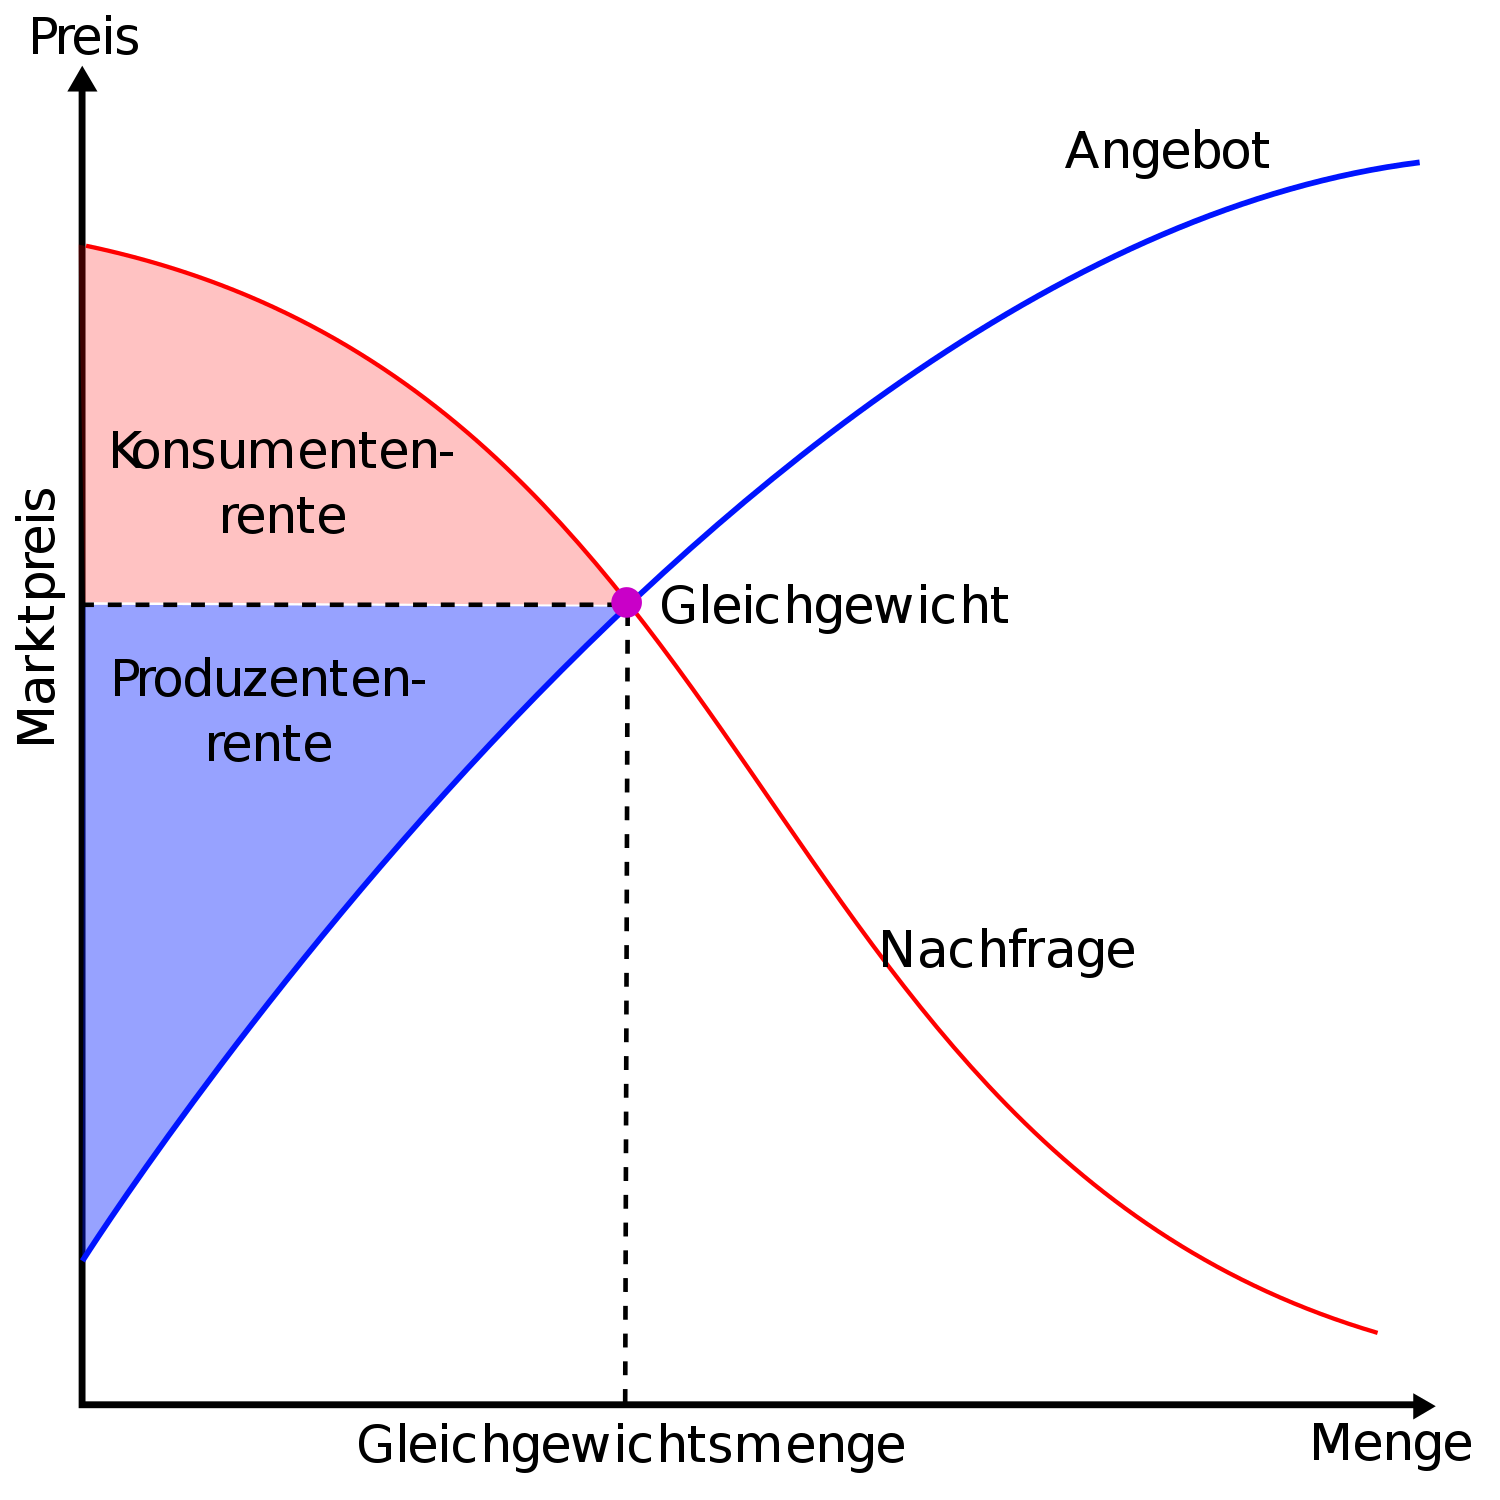
\includegraphics[width=0.4\textwidth]{bilder/wohlfahrt.png}
\end{center}

\section{Wirtschaftsordnungen}
% TODO
// Nicht klausurrelevant, ausgelassen

\section{Unternehmen}
\subsection{Der Unternehmer}
\subsubsection{Ronald Coase}
Nach Coase sind Unternehmer Organisatoren, da sie Transaktionskosten, die bei der Suche nach den günstigsten Preisen am Markt entstehen, durch lang anhaltende Verträge mindern.

\subsubsection{Karl Marx}
$\Rightarrow$ \textbf{Koordinierender Teil} des Wirtschaftsgeschehens
Nach Marx können Unternehmer nur \textbf{ausbeuten}, da die Geschicklichkeit der Konkurrenz durch neue Produktionsmöglichkeiten entwertet wird. Er sagt: \enquote{Die in [der Gesellschaft] arbeiten, erwerben nicht, und die in ihr erwerben, arbeiten nicht}.

$\Rightarrow$ \textbf{Abschöpfender Teil} des Wirtschaftsgeschehens


\subsubsection{Joseph Schumpeter}
Durch dir Überwindung der Routine wird der Kreislauf der Gewohnheit durchbrochen und es entsteht Neues. Der Prozess, neue Möglichkeiten zu erkennen und durchzusetzen ist der Hauptgrund für die wirtschaftliche Entwicklung. Dieser Prozess heißt \textbf{schöpferischer Zer\-stö\-rungs\-pro\-zess}. Die Aufgabe der Unternehmer ist somit, \textbf{Neuerungen zu entdecken und durchzusetzen}. Dies geschieht folgendermaßen:

\begin{itemize}
    \item Herstellung eines neuen Gutes
    \item Einführung einer neuen Produktionsmethode
    \item Erschließung eines neuen Absatzmarkts
    \item Eroberung einer neuen Bezugsquelle
    \item Neuorganisation, z.B. Monopol
\end{itemize}
Unternehmer genießen jedoch nicht den Erfolg, sondern schaffen rastlos.

$\Rightarrow$ \textbf{Aktiver \& kreativer Teil} des Wirtschaftsgeschehens


\subsection{Kondratjew-Zyklen}
\subsubsection{Erklärung}
\textbf{Kondratjew-Zyklen} sind gesamtwirtschaftliche Zyklen, die jeweils mit \textbf{Basisinnovationen} starten, aufgrund derer die Produktivität steigt. Dieser \textbf{Produktivitätszuwachs} endet, wenn eine produktivitätsbeschränkende Schwelle erreicht wird. Daraufhin wird die \textbf{Realkostengrenze} gesucht, die durch eine weitere Basisinnovation beseitigt werden kann.

\subsubsection{Bisherige Zyklen}
\begin{tabular}{|l|l|} \hline
    Nummer & Basisinnovation \\ \hline
    1 & Dampfmaschine, Textilindustie \\ \hline
    2 & Eisenbahn, Massentransport \\ \hline
    3 & Strom, Massenproduktion \\ \hline
    4 & Auto, individuelle Mobilität \\ \hline
    5 & Informationstechnik, strukturierte Information \\ \hline
    6 & ??? \\ \hline
\end{tabular}

\subsection{Unternehmungen vs. Betriebe}
\begin{tabularx}{\textwidth}{|l|X|X|} \hline
    & Betrieb & Unternehmung \\ \hline
    Bestandteile & Produktionsstätte & Produktionsstätte, Rechtsform, Kapital \\ \hline
    Aufgaben & Bereitstellung von Sachgütern und Dienstleistungen & Gewinnerzielung, Schaffung der Produktionsvorausstzungen \\ \hline
    Besonderheiten & Können keine eigenen Entscheidungen treffen, Preise etc. werden von zentralen Planungsbehörden festgelegt. & Können mehrere Betriebe haben \\ \hline
\end{tabularx}

\subsection{Betriebsarten}
Klassifizierung nach Betriebsgröße:

\begin{tabular}{|c|l|} \hline
    Anzahl an Beschäftigten & Betriebsgröße \\ \hline
    $\le20$ & Kleinstbetrieb  \\ \hline
    $20-100$ & Kleinbetrieb \\ \hline
    $100-1000$ & Mittelbetrieb \\ \hline
    $\ge1000$ & Großbetrieb \\ \hline
\end{tabular}

Klassifizierung nach Tätigkeit, man unterscheidet
\begin{itemize}
    \item \textbf{Urproduktionsbetriebe}, z.B. Landwirtschaft, Fischerei, Forst
    \item \textbf{Verarbeitungsbetriebe}, z.B. Fabriken, Schreinerei
    \item \textbf{Dienstleistungsbetriebe}, z.B. Fluggesellschaft, Versicherung
    \item \textbf{Handelsbetriebe}, z.B. Lebensmittelgeschäfte
\end{itemize}

Urproduktionsbetriebe und Verarbeitungsbetriebe werden auch \textbf{Produktionsbetriebe} genannt.


\subsection{Rechtsformen}

\subsubsection{Personengesellschaften}
\paragraph{Einzelunternehmung}
\begin{itemize}
    \item Eine natürliche Person (Firmenname: Name des Inhabers)
    \item Automatisch ohne eine angegebene Rechtsform
    \item Vollständiger Gewinn und Verlust gehört Unternehmer
    \item Haftung mit vollständigem Geschäfts- und Privatvermögen
\end{itemize}
% Eine Einzelunternehmung wird von einer natürlichen Person gegründet und heißt wie sie selbst. Ohne eine angegebene Rechtsform ist ein Unternehmen eine Einzelunternehmung. Der vollständige Gewinn und Verlust gehört dem Unternehmer, er haftet mit seinem gesamten Geschäfts- und Privatvermögen.

\paragraph{GbR (Gesellschaft bürgerlichen Rechts) oder auch BGB-Gesellschaft}
\begin{itemize}
    \item Gründung durch mehrere natürliche Personen durch (auch formfreien) Gesellschaftsvertrag
    \item Mindestkapital: 0€
    \item Haftung mit vollständigem Geschäfts- und Privatvermögen
    \item Verteilung des Gewinns nach Köpfen
    \item Führung: Gemeinsam
    \item Vorteile: Einfache Gründung
    \item Keine Eintragung im Handelsregister
\end{itemize}
% Eine GbR ist ein Zusammenschluss mehrerer natürlicher Personen durch einen (auch formfreien) Gesellschaftsvertrag (Mindestkapital 0€). Der Gewinn und Verlust wird aufgeteilt, die Haftung geschieht durch das vollständige Geschäfts- und Privatvermögen der Gesellschafter. Vorteil einer GbR ist die einfache Gründung, jedoch besteht auch eine hohe Haftung. Eine GbR ist nicht im Handelsregister eingetragen.

\paragraph{OHG (Offene Handelsgesellschaft)}
\begin{itemize}
    \item Unternehmung muss Handelsunternehmung sein
    \item Zusammenschluss von mindestens zwei natürlichen Personen durch Gesellschaftsvertrag
    \item Gewinn: 4\% des Kapitalanteils + Rest nach Köpfen
    \item Verlust: Verteilung nach Köpfen
    \item Haftung mit vollständigem Geschäfts- und Privatvermögen
    \item Führung: Gemeinsam
    \item Vorteile: Hohes Ansehen bei Kapitalgebern
    \item Eintragung ins Handelsregister
\end{itemize}
% Eine OHG wird durch einen Gesellschaftsvertrag zwischen Kaufmännern gegründet (Mindestkapital 0€), sodass das Unternehmen nur im kaufmännischen Bereich tätig sein kann. Als Gewinn wird 4\% des Kapitalanteils vergütet, der Rest wird nach Köpfen verteilt. Der Verlust wird auch nach Köpfen veteilt. Wie auch bei der GbR wird ungeschränkt mit dem gesamten Geschäfts- und Privatvermögen gehaftet. Die OHG muss im Handelsregister eingetragen sein.

\paragraph{KG (Kommanditgesellschaft)}
\begin{itemize}
    \item Gründung durch mindestens zwei natürlichen Personen (ein Komplementär, ein Kommanditist) 
    \item Mindestkapital: 0€
    \item Komplementär $\rightarrow$ Vollhafter, Haftung mit gesamtem Geschäft- und Privatvermögen $\rightarrow$ Geschäftsführung, Entscheidungsrecht
    \item Kommanditist $\rightarrow$ Teilhafter, Haftung mit Kapitaleinlage $\rightarrow$ Widerspruchsrecht, Kontrollrecht
    \item Gewinnverteilung: 4\% der Kapitaleinlage + Rest nach Risikoanteilen
    \item Verlustverteilung: Nach angemessenen Anteilen
    \item Vorteile: Einfache Kapitalaufnahme, da Gesellschafter nicht haften muss
    \item Eintragung ins Handelsregister
\end{itemize}
% Eine Kommanditgesellschaft wird von mindestens zwei Personen gegründet (Mindestkapital 0€), um ein Handelsgewerbe zu betreiben. Besonders ist, dass mindestens eine Person \textbf{Komplementär} (Vollhafter) ist, die die Geschäftsleitung stellt, jedoch auch mit ihrem gesamten Geschäfts- und Privatvermögen haften. Die \textbf{Kommanditist}en sind zwar Gesellschafter, überlassen aber den Komplementären die Geschäftsleitung, haften dafür aber nicht mit ihrem Privatvermögen. Sie verfügen über ein Kontrollrecht und ein Widerspruchsrecht bei außergewöhnlichen Geschäftsvorgängen. Die Gewinnverteilung ist 4\% der Kapitaleinlage und restliche Verteilung nach Risikoanteilen. Der Verlust wird nach angemessenen Anteilen verteilt. Der Vorteil der KG ist, dass Kapitalgewinnung durch die Haftungsbeschränkung vereinfacht ist. Die KG muss im Handelsregister eingetragen sein.

\subsubsection{Kapitalgesellschaften}
\paragraph{Gesellschaft mit beschränkter Haftung (GmbH)}
\begin{itemize}
    \item Gründung: Mindestens eine natürliche Person, notarielle Bekundigung
    \item Mindestkapital: 25000€, bei Unternehmergesellschaft: 1€
    \item Führung: Geschäftsführer
    \item Haftung mit Kapitaleinlage
    \item Vorteile: Geschäftsführer muss nicht Gesellschafter sein, keine Haftung
    \item Nachteile: Erschwerte Kapitalaufnahme
    \item Eintragung ins Handelsregister
\end{itemize}
% Eine GmbH wird von einer natürlichen Person mit 25000€ Mindestkapital mit notarieller Bekundigung gegründet (Unternehmergesellschaft: 1€). Die Führung erfolgt durch den Geschäftsführer, der nicht Gesellschafter sein muss. Gehaftet wird mit dem Gesellschaftsvermögen. Gewinn und Verlust wird entsprechend der Anteile verteilt. Vorteile der GmbH sind, dass der Geschäftsführer nicht Gesellschafter sein muss und dass keine Haftung besteht. Durch die beschränkte Haftung ist jedoch z.B. eine Kreditaufnahme erschwert. Die GmbH muss im Handelsregister eingetragen sein.

\paragraph{Aktiengesellschaft (AG)}
\begin{itemize}
    \item Gründung: Mindestens eine natürliche Person, notarielle Bekundigung
    \item Mindestkapital: 50000€
    \item Führung: Vorstand, Kontrolle durch Aufsichtsrat
    \item Gewinn: Verteilung über Dividende
    \item Haftung: Durch Aktie
    \item Aktionäre haben Teilnahme- und Stimmrecht an Hauptversammlungen, sowie Dividendenrecht
    \item Vorteile: Eignung für große Unternehmung durch einfache Kapitalgewinnung
    \item Eintragung ins Handelsregister
\end{itemize}
% Eine Aktiengesellschaft kann von einer natürlichen Person mit 50000€ Mindestkapital mit notarieller Bekundigung gegründet werden. Die Führung erfolgt durch den Vorstand, der vom Aufsichtsrat kontrolliert wird. Der Gewinn wird durch die Dividende an \textbf{Aktionäre} verteilt, gehaftet wird über die Aktie. Aktionäre haben das Dividendenrecht und das Teilnahmerecht an Hauptversammlungen. Die Rechtsform der AG ist für große Unternehmen geeignet, da Kapitalgewinnung durch Aktien vereinfacht wird. Eine AG muss im Handelsregister eingetragen werden.


\subsection{Rechnungswesen}
\subsubsection{Bilanz}
\begin{itemize}
    \item Zeitpunktbetrachtung $\rightarrow$ Stichtag angeben!
    \item Sagt aus, wie viel das Unternehmen wert ist
    \item Zeigt Vermögen (Aktiva) und Finanzierung (Passiva) auf
    \item Summe der Aktiva und Passiva muss gleich sein $\rightarrow$ Bilanzsumme
    \item Aktiva sind aufsteigend nach Liquidität geordnet (Gliederung in Anlage- und Umlaufvermögen)
    \item Passiva sind absteigend nach Fristigkeit geordnet (Gliederung in Eigen- und Fremdkapital)
\end{itemize}

\textbf{Beispiel:}

\begin{tabularx}{\textwidth}{|X|l|X|l|} \hline
    \textbf{Aktiva} & & \textbf{Passiva} & \\ \hline
    \textbf{Anlagevermögen} & & \textbf{Eigenkapital} & 1000€ \\ \hline
    Immaterielle Vermögensgegenstände & 100€ & \textbf{Fremdkapital} & \\ \hline
    Einrichtung & 5000€ & Langfristige Verbindlichkeiten & 4000€ \\ \hline
    Fahrrad & 300€ & Lieferverbindlichkeiten & 3000€ \\ \hline
    \textbf{Umlaufvermögen} & & & \\ \hline
    Rohstoffe & 300€ & & \\ \hline
    Kasse & 1900€ & & \\ \hline
    \textbf{Bilanzsumme} & 8000€ & \textbf{Bilanzsumme} & 8000€ \\ \hline
\end{tabularx}

\subsubsection{GuV}
\begin{itemize}
    \item Stellt Gewinn und Verlust des Jahres gegenüber
    \item Erträge -- Aufwendungen 
    \item Es kann erkannt werden, woher der Gewinn und Verlust kommt
    \item Äquivalent zu Eigenkapital - Eigenkapital Vorjahr
\end{itemize}


\subsubsection{Kennzahlen}

\paragraph{Eigenkapitalquote / Grad der finanziellen Unabhängigkeit}
$$ \textrm{EKQ} = \frac{\textrm{Eigenkapital}}{\textrm{Gesamtkapital}} * 100\% $$

\paragraph{Fremdkapitalquote / Anspannungsgrad}
$$ \textrm{FKQ} = \frac{\textrm{Fremdkapital}}{\textrm{Gesamtkapital}} * 100\% $$

\paragraph{Verschuldungsgrad}
$$ \textrm{Verschuldungsgrad} = \frac{\textrm{Fremdkapital}}{\textrm{Eigenkapital}} * 100\% $$

\paragraph{Anlagenintensität}
$$ \textrm{Anlagenintensität} = \frac{\textrm{Anlagevermögen}}{\textrm{Gesamtvermögen}} * 100\% $$

\paragraph{Vorratsintensität}
$$ \textrm{Vorratsintensität} = \frac{\textrm{Vorratsvermögen}}{\textrm{Gesamtvermögen}} * 100\% $$

\paragraph{Eigenkapitalrentabilität}
$$ \textrm{EKR} = \frac{\textrm{Gewinn}}{\textrm{Eigenkapital}} * 100\% $$

\paragraph{Produktivität}
$$ \textrm{Produktivität} = \frac{\textrm{Ausbringungsmenge}}{\textrm{Einsatzmenge}} $$

\subsubsection{Der Leverage-Effekt}
\begin{itemize}
    \item Aufnahme von Fremdkapital zur Steigerung der Eigenkapitalrendite
    \item Möglich, wenn Fremdkapitalzins $<$ Gesamtkapitalrentabilität
    \item Bei Ersatz von Eigenkapital durch Fremdkapital sinkt Gesamtgewinn
    \item Leverage-Effekt wirkt als Hebel in beide Richtungen $\rightarrow$ Rentabilität kann auch sinken
    \item Kann nicht unendlich fortgeführt werden $\rightarrow$ Bonität des Unternehmens sinkt
\end{itemize}

\subsubsection{Grundformen der Unternehmensfinanzierung}
\begin{tabular}{|l|l|l|}\hline
    & \textbf{Eigenkapital} & \textbf{Fremdkapital} \\ \hline
    \textbf{Außenfinanzierung} & Beteiligungsfinanzierung & Kreditfinanzierung \\ \hline
    \textbf{Innenfinanzierung} & Selbstfinanzierung & Rückstellungen \\ \hline
\end{tabular}

\subsection{Betriebliche Grundfunktionen}
\begin{itemize}
    \item Leitungsfunktion
    \item Beschaffungsfunktion
    \item Fertigungsfunktion
    \item Absatzfunktion
    \item Finanzierungsfunktion / Rechnungswesen
\end{itemize}

\subsection{Ziele}
\begin{tabularx}{\textwidth}{|l|X|X|} \hline
    Art & Öffentliche Unternehmung & Privatunternehmung \\ \hline
    Hauptziel & Bedarfsdeckung & Erwirtschaftung von Gewinn \\ \hline
Weitere Ziele & 
\begin{itemize}
    \item angemessener Gewinn
    \item Verlustminimierung
    \item Kostendeckung
\end{itemize}
    & 
    \begin{itemize}
        \item Steigerung der Leistung
        \item Firmenimage
        \item Produktivität
        \item Steigerung der Rentabilität
        \item Hoher Marktanteil
        \item Arbeitsplatzsicherheit
    \end{itemize}
    \\ \hline
\end{tabularx}

\subsubsection{Der Stakeholder-Ansatz}
\begin{itemize}
    \item Ansatz beim Treffen von Entscheidungen
    \item Berücksichtigung aller Interessensgruppen am Unternehmen, z.B. Eigentümer, Kunden, Arbeitnehmer, Staat und Öffentlichkeit, Lieferanten oder Banken
    \item Interessenskonflikte möglich!
\end{itemize}

\subsection{Produktionsfaktoren}
\subsubsection{Betriebswirtschaftliche Produktionsfaktoren}
\begin{itemize}
    \item \textbf{Betriebsmittel} sind an der Produktion beteiligt und werden nicht verbraucht, fließen aber nicht direkt darin ein, z.B. Maschinen, Werkzeuge oder Produktionsgebäude
    \item \textbf{Werkstoffe} fließen in das Produkt mit ein. Sie werden unterteilt in
    \begin{itemize}
        \item Rohstoffe, z.B. Holzbretter
        \item Hilfsstoffe, z.B. Lack, Holzleim
        \item Betriebsstoffe, z.B. Strom, Schmieröl
        \item Bezogene Fertigteile
    \end{itemize}
    \item \textbf{Arbeit}
\end{itemize}
Die Anteile der Produktionsfaktoren müssen wegen ihrer Preisänderung ständig angepasst werden.
\subsubsection{Volkswirtschaftliche Produktionsfaktoren}
\begin{itemize}
    \item Boden
    \item Arbeit
    \item Kapital
    \item (Information)
\end{itemize}

\subsection{CSR}
\textbf{Corporate Social Responsibility}
\begin{itemize}
    \item Übernahme sozialer Verantwortung durch Unternehmen
    \item Nicht nur Pflicht, sondern auch Investitionen, die sich in der Wertschöpfung niederschlagen
    \item Nachhaltiges Wachstum, Wettbewerbsvorteilen, höhere Reputation
    \item Muss über gesetzliche Vorgaben hinausgehen
\end{itemize}

\subsubsection{Unternehmensleitbilder}
\begin{itemize}
    \item Reflektiert Wertebasis eines Unternehmens, grundlegende Überzeugungen, Ziele und Verantwortung gegenüber Stakeholdern
    \item Verschaffen intern Orientierung und Identität
    \item Vermitteln extern Transparenz und Bereitschaft zu CSR
    \item Senken Anteil wirtschaftskrimineller Handlungen
    \item Strafen wegen Fehlverhalten Einzelner können vermindert werden
\end{itemize}

\subsubsection{Greenwashing}
\textbf{Greenwashing} bezeichnet den Versuch von Unternehmen, durch Marketingmaßnahmen ein \enquote{grünes} Image zu erlangen, ohne entsprechende Maßnahmen in der Wertschöpfung zu implementieren.

\subsection{Lean Production}
\begin{itemize}
    \item Fokussierung aller Prozesse auf die Wertschöpfung
    \item Übergabe eines Maximums an Aufgaben und Verantwortlichkeiten an die Mitarbeiter
    \item Frühzeitige Fehlerentdeckung und -behebung
    \item Just-In-Time-Zulieferung
\end{itemize}
$\Rightarrow$ Optimierung der Wertschöpfung, Reduktion der Komplexität bei den Beteiligten


\section{Marketing}
\begin{itemize}
    \item Alle unternehmerischen Aktivitäten, die auf den Markt, bzw. den Kunden ausgerichtet sind.
    \item Grund: Angebot größer als Nachfrage (Käufermarkt)
    \item Marktorientierte Unternehmensführung: Ausrichtung aller Aktivitäten auf die heutigen und zukünftigen Märkte und Wettbewerber
    \item Sowohl Unternehmensfunktion als auch Leitkonzept des Managements
\end{itemize}

\subsection{Produktlebenszyklus}
\begin{itemize}
    \item Kann auf Einzelne Produkte, Produktformen oder ganze Produktklassen angewendet werden
    \item Lebenszyklen einzelner Produkte sind stark abhängig von der Reaktion der Konkurrenz
\end{itemize}


\begin{tabularx}{\textwidth}{|r|l|X|} \hline
    & Phase & Beschreibung \\ \hline
    1 & Entwicklungsphase & 
    \begin{itemize}[noitemsep]
        \item Hohe Investitionen für Produktentwicklung
        \item Keine Verkaufserlöse
    \end{itemize} \\ \hline
    2 & Einführungsphase & 
    \begin{itemize}[noitemsep]
        \item Absatz wächst langsam
        \item Noch keine Gewinne
        \item Hohe Marketingausgaben zur Steigerung der Bekanntheit
    \end{itemize} \\ \hline
    3 & Wachstumsphase & 
    \begin{itemize}[noitemsep]
        \item Produkt wird am Markt akzeptiert
        \item Absatz steigt deutlich
        \item Nachfragesteigerung durch Wiederholungskäufe
        \item Erreichen der Gewinnzone
    \end{itemize} \\ \hline
    4 & Reifephase und Sättigungsphase & 
    \begin{itemize}[noitemsep]
        \item Umsatz und Markt wächst, Zuwachsraten nehmen jedoch ab
        \item Kaum Neukunden
        \item Auftreten von Konkurrenz und Imitationen $\rightarrow$ Steigerung des Marketings
        \item Marktsättigung gegen Ende
    \end{itemize} \\ \hline
    5 & Degenerationsphase & 
    \begin{itemize}[noitemsep]
        \item Viele Imitationen von gleicher Qualität und Preis
        \item Stark sinkender Umsatz
        \item Auslaufen und Ersetzen durch Nachfolgeprodukt
    \end{itemize} \\ \hline
\end{tabularx}

\begin{center}
    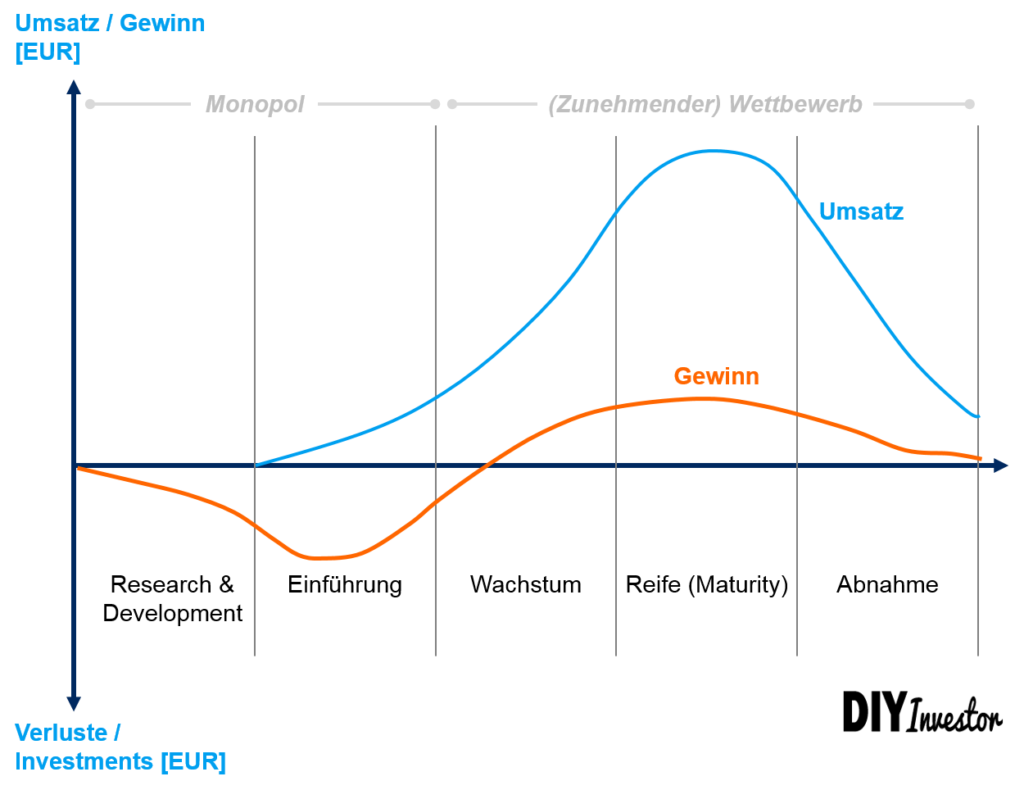
\includegraphics[width=0.85\textwidth]{bilder/produktlebenszyklus.png}
\end{center}

\subsection{Portfolio-Analyse (BCG)}
\begin{itemize}
    \item Analysiert Marktanteil und Marktwachstum von Produkten eines Unternehmens
    \item Zwei Achsen: Marktanteil und Marktwachstum
    \item Unterteilung der Produkte in \textbf{Poor Dogs}, \textbf{Cash Cows}, \textbf{Stars} und \textbf{Question Marks}
\end{itemize}

\begin{center}
    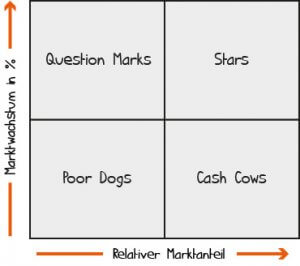
\includegraphics[width=0.5\textwidth]{bilder/portfolioanalyse.jpg}
\end{center}

\begin{tabularx}{\textwidth}{|l|l|l|l|X|} \hline
    Name & Marktanteil & Wachstum & Investitionsbedarf & Anderes \\ \hline
    Poor Dogs & niedrig & niedrig & niedrig & selbsterhaltend aber ohne Zukunft \\ \hline
    Cash Cows & hoch & niedrig & gering & \enquote{Geldbringer} \\ \hline
    Stars & hoch & hoch & hoch & Werden oft \enquote{Cash Cows} \\ \hline
    Question Marks & niedrig & hoch & hoch & Zum \enquote{Star} entwickeln oder aufgeben \\ \hline
\end{tabularx}



\subsection{SWOT-Analyse}
\begin{itemize}
    \item Analyse von Stärken, Schwächen, Möglichkeiten und Risiken eines Unternehmens
    \item Stärken und Schwächen kommen von innen (\textbf{interne Analyse}), Möglichkeiten und Risiken von außen (Markt) \textbf{externe Analyse}
\end{itemize}

\subsection{Marktforschung}
Zwei Arten der Marktforschung:
\begin{enumerate}
    \item \textbf{Primärforschung} $\rightarrow$ Erhebung neuer Daten
    \item \textbf{Sekundärforschung} $\rightarrow$ Auswertung vorhandenen Datenmaterials
\end{enumerate}

\subsection{Der Marketing-Mix}
\subsubsection{Product}
Im Rahmen der \textbf{Produktpolitik} legen Unternehmer die Produkteigenschaften fest. Dabei stehen verschiedene Maßnahmen zur Auswahl:
\begin{itemize}
    \item Produktinnovation
    \item Produktdiversifikation
    \item Produktdifferenzierung oder -variation
    \item Produkteliminierung
\end{itemize}

\subsubsection{Place}
Im Rahmen der \textbf{Distributionspolitik} wird festgelegt, wo das Produkt in welcher Menge zur Verfügung stehen soll. Dabei sind verschiedene Absatzwege und Vertriebssysteme zu unterscheiden:

\paragraph{Absatzwege}
\begin{itemize}
    \item Direkter Absatzweg, Verkauf direkt an den Verbraucher (B2C)
    \item Indirekter Absatzweg, Verkauf über Mittler (B2B)
\end{itemize}

\paragraph{Vertriebssysteme}
\begin{itemize}
    \item \textbf{Vertragshändlersystem} $\rightarrow$ Verkauf auf eigenen Namen und eigene Rechnung, Durch\-füh\-rung von Kundendiensten, Mindestabgabemenge
    \item \textbf{Franchising} $\rightarrow$ Engere Bindung, Keine eigene Firma, Franchisenehmer übernimmt marketingpolitische Vorgaben
\end{itemize}

Heutzutage werden auch Telefonmarketing, Online-Shops oder Virtuelle Marktplätze wie ebay zur Distribution verwendet.

\subsubsection{Price}
Die \textbf{Preis- und Konditionenpolitik} kennt viele Gestaltungsmöglichkeiten:

\paragraph{Preisfindung}
\begin{itemize}
    \item Kostenorientierung (Preisuntergrenze)
    \item Marktorientierung (Preisobergrenze) $\rightarrow$ Wettbewerbs- oder kundenorientiert
\end{itemize}

\paragraph{Preisstrategie}
\begin{itemize}
    \item Festpreisstrategie, niedrig oder hoch $rightarrow$ Markt- oder Qualitätsführung
    \item Preisabfolgestrategie $\rightarrow$ langsame Veränderung des Preises:
    \begin{itemize}
        \item Abschöpfungsstrategie $\rightarrow$ Mit hohem Preis anfangen
        \item Penetrationsstrategie $\rightarrow$ Mit niedrigem Preis anfangen
    \end{itemize}
    \item Preisdifferenzierung $\rightarrow$ Absetzen des Produkts zu verschiedenen Preisen
\end{itemize}

\paragraph{Konditionenpolitik}
Rabatte und Boni, Lieferungsbedingungen, Zahlungsbedingungen


\subsubsection{Promotion}
Ziel der \textbf{Kommunikationspolitik} ist die Wahrnehmung des Produkts von der Zielgruppe. Dies geschieht durch:
\begin{itemize}
    \item Werbung
    \item Verkaufsförderung
    \item Öffentlichkeitsarbeit (Public Relations)
    \item Sponsoring
    \item Product Placement
\end{itemize}

\subsection{Marketing-Controlling}
Marketing-Controlling ist zuständig für:
\begin{itemize}
    \item Koordinierung und Kontrolle der Marktforschung und Wettbewerbsanalyse
    \item Möglichst frühzeitige Informierung der Strategieplanung über Ereignisse
    \item Ausführen der von der Strategieplanung vorgegebenen Strategie
    \item Erstellen von Plänen für Marketingmaßnahmen
\end{itemize}

\subsection{Grenzen des Marketings}
Das \textbf{Gesetz gegen den unlauteren Wettbewerb} (UWG) setzt der Werbung in Deutschland Grenzen. Verboten sind beispielsweise:
\begin{itemize}
    \item Schleichwerbung
    \item Herabsetzung des Konkurrenten
    \item Irreführende Werbung
    \item Verkaufsförderung durch Gewinnspiele
    \item Unzumutbare Belästigungen
\end{itemize}

Weiterhin gibt es einige psychologische Effekte, die die Wirkung von Werbung reduziert:
\begin{itemize}
    \item \textbf{Ablenkungseffekt}: Gestalterische Elemente lenken vom Inhalt ab
    \item \textbf{Carry-over-Effekt}: Ökonomische Wirkung ist zeitversetzt und deshalb nur schwer Maßnahmen zurechenbar
    \item \textbf{Information-Overload}
    \item \textbf{Overpromising}
    \item \textbf{Sleeper-Effekt}: Gestalterische Inhalte bleiben mehr im Gedächtnis als Marke
    \item \textbf{Wear-Out-Effekt}: Abnutzung der Werbung, Auslösen von Ermündung oder Protesthaltungen
\end{itemize}

\section{Der Mitarbeiter im Unternehmen}
% TODO
// Nicht klausurrelevant, ausgelassen

\section{Staat}
\subsection{Das magische Viereck}
\begin{itemize}
    \item 4 wichtige Aspekte der Wirtschaftspolitik
    \item Schwierig, alle gleichzeitig zu erfüllen
    \item Hoher Beschäftigungsgrad, Preisniveaustabilität, Angemessenes und stetiges Wirtschaftswachstum, Ausgeglichene Außenhandelsbilanz
\end{itemize}

\subsubsection{Hoher Beschäftigungsgrad}
\begin{itemize}
    \item Ziel: Vollbeschäftigung
    \item Indikator: Arbeitslosenquote
    \begin{itemize}
        \item In Deutschland: \textbf{arbeitslos}: keine Arbeit oder $<15$ h pro Woche, sich bei der Bundesagentur für Arbeit gemeldet, vermittelbar (Sozialgesetzbuch)
        \item International (ILO): \textbf{erwerbslos}: ohne Arbeit, verfügbar und auf Suche $\rightarrow$ international vergleichbar
    \end{itemize}
    \item Tatsächliche Arbeitslose:
    \begin{itemize}
        \item + über 58-jährige ohne Jobangebot seit 12 Monaten
        \item + kurzfristig Arbeitsunfähige (krankgeschrieben)
        \item + Teilnehmer an arbeitsmarktpolitischen Maßnahmen
    \end{itemize}
    \item Vorteile niedriger Arbeitslosigkeit:
    \begin{itemize}
        \item Geringere Kosten
        \item Höhere Zufriedenheit
        \item Höheres Wirtschaftswachstum
    \end{itemize}
    \item Nachteile niedriger Arbeitslosigkeit:
    \begin{itemize}
        \item Fachkräftemangel
        \item Zu wenig Arbeitnehmer
        \item (ungleiche Verteilung)
    \end{itemize}
    \item Formen der Arbeitslosigkeit:
    \begin{itemize}
        \item "Bodensatz" (unvermittelbar)
        \item Friktionelle Arbeitslosigkeit
        \item Konjunkturelle Arbeitslosigkeit
        \item Saisonale Arbeitslosigkeit
        \item Strukturelle Arbeitslosigkeit
    \end{itemize}
\end{itemize}

\subsubsection{Preisniveaustabilität}
\begin{itemize}
    \item Ziel: Inflation von ca. 2\% pro Jahr
    \item Indikator: Inflationsrate
    \begin{itemize}
        \item Preisliche Veränderung eines repräsentativen Warenkorbs $\rightarrow$ Verbraucherpreisindex (HVPI)
        \item $\mathrm{Inflationsrate}_x = \frac{\mathrm{Preis}_{x+1}}{\mathrm{Preis}_x}$
    \end{itemize}
    \item \textbf{Inflation}: Anhaltender Prozess der Geldentwertung, d.h. eine dauerhafte Kaufkraftverminderung
    \item Selbstverstärkung durch Lohn-Preis-Spirale
    \item Bevorteiligt durch hohe Inflation: Schuldner, Besitzer von Anlagen wie Aktien, Rohstoffe, Immobilien
    \item Benachteiligt durch hohe Inflation (\textbf{Kaufkraftverlust}): Arbeitslose, Rentner, Bezieher von Sozialleistungen, Kleinsparer
    \item Ursache: 
    \begin{itemize}
        \item Geldmenge steigt
        \item Knappheit steigt
    \end{itemize}
\end{itemize}

\subsubsection{Angemessenens und stetiges Wirtschaftswachstum}
\begin{itemize}
    \item Ziel: Stetiges und angemessenes Wirtschaftswachstum
    \begin{itemize}
        \item Vermeidung von konjukturellen Schwankungen
        \item Ausreichendes Wachstum für hohen Beschäftigungsgrad in der Zukunft.
    \end{itemize}
    \item Indikator: \textbf{Bruttoinlandsprodukt}: 
    \begin{itemize}
        \item Marktwert aller für den Endverbrauch bestimmten Produkte und Dienstleistungen, die in einem Land über einen bestimmten Zeitraum hergestellt werden.
        \item Misst Wertschöpfung in einem Land über einen Zeitraum
        \item \textbf{Entstehungsrechnung}: In welchen Sektoren entsteht die Wertschöpfung?
        \item \textbf{Verwendungsrechnung}: Private und staatliche Konsumaufgaben, Investitionen, Außenbeitrag
        \item \textbf{Verteilungsrechnung}: Volkseinkommen, Produktions- und Importabgaben an den Staat (abzüglich Subventionen), Abschreibungen, Saldo der Primäreinkommen aus der übrigen Welt
        \item Kritik: 
        \begin{itemize}
            \item BIP nicht als Wohlstandsindikator gedacht $\rightarrow$ Orientierung am Wachstum nicht unbedingt sinnvoll
            \item Berücksichtigt keine sozialen Aspekte (Bildung etc.), Einkommensverteilung, Ökologie, Lebenserwartung, Kriminalität etc.
            \item Freizeit und Ehrenamt nicht berücksichtigt
            \item Alternativen: NWI, HDI
        \end{itemize}
    \end{itemize}
    \item $\mathrm{Wachstum}_{\mathrm{nominell},x,x+1} = \frac{\mathrm{BIP}_{x+1}}{\mathrm{BIP}_{x}} * 100\%$
    \item $\mathrm{Wachstum}_{\mathrm{real},x,x+1} = \frac{\mathrm{Wachstum}_{\mathrm{nominell},x,x+1}}{\mathrm{Inflation}} * 100\%$
\end{itemize}

\subsubsection{Ausgeglichene Außenhandelsbilanz}
\begin{itemize}
    \item Ziel: Ausgeglichene Importe und Exporte
    \item Indikator: Leistungs-, Handels- und Kapitalbilanz
    \begin{itemize}
        \item Leistungsbilanz: Exporte und Importe an Waren und Dienstleistungen 
        \item Handelsbilanz: Exporte und Importe von Waren
        \item Kapitalbilanz: Zu- und Abflüsse an Kapital
        \item i.d.R. sind Leistungs- und Kapitalbilanz entgegengesetzt
    \end{itemize}
    \item In Deutschland: Kapitaltalbilanz seit 1950er positiv, Leistungsbilanz seit 2002
\end{itemize}

\subsubsection{Magisches Vieleck}
Magisches Viereck plus:
\begin{itemize}
    \item Soziale Gerechtigkeit (GG Art. 1 + Art. 20)
    \item Umweltschutz (GG Art. 20a)
\end{itemize}

\subsection{Konjunktur}
\begin{itemize}
    \item Kurz- und mittelfristige Schwankungen im Wirtschaftswachstum einer Volkswirtschaft
    \item Konjunkturelle Schwankungen $\Leftrightarrow$ Strukturelle Schwankungen (z.B. Kondratjew)
    \item 4 Phasen: Aufschwung, Boom, Rezession, Depression
    \item Konjukturindikatoren:
    \begin{itemize}
        \item \textbf{Frühindikatoren}: Geschäftsklimaindex, Auftragseingänge, Baugenehmigungen
        \item \textbf{Präsensindikatoren}: Kapazitätsauslastung, Produktionsindex, Handelsbilanz
        \item \textbf{Spätindikatoren}: Arbeitsmarkt, Bruttoinlandsprodukt, Preisindex
    \end{itemize}
\end{itemize}

\subsubsection{Ursachen}
Verschiedene Theorien:
\begin{itemize}
    \item \textbf{Monetäre Theorien}: Zurückführung auf monetäre Faktoren (Geldmenge, Zins)
    \item \textbf{Überinvestitionstheorie}: Rezession durch übermäßige Ausdehnung ds Investitionsgütersektors im Aufschwung
    \item \textbf{Unterkonsumtionstheorie}: Im Boom bleibt Konsumgüternachfrage hinter Produktionsmöglichkeiten zurück, da Löhne und Gehälter nicht in gleichem Ausmaß steigen wie Güterpreise und Gewinne
    \item \textbf{Exogene Theorien}: Faktoren, die nicht direkt durch as Wirtschaftsgeschehen beeinflusst werden, z.B. Naturkatastrophen, Kriege, Erfindungen
\end{itemize}

\subsection{Wirtschaftspolitische Ansätze}
\subsubsection{Keynesianismus}
\begin{itemize}
    \item Für Intervention des Staates in den Wirtschaftskreislauf
    \item \textbf{Liquiditätsfalle}: Durch Angst der Unternehmer "verschwindet" Geld aus dem Kreislauf und wird gehortet $\rightarrow$ Investitionslücke
    \item Antizyklische Fiskalpolitik
    \item \textbf{deficit spending}: Steuersenkungen und höhere Staatsausgaben (kreditfinanziert) in der Rezession $\rightarrow$ Erhöhung der Nachfrage
    \item Finanzierung durch Steuererhöhungen und Sparsamkeit im Boom
    \item \textbf{Multiplikatoreffekt}: Erhöhung der Nachfrage durch den Staat $\rightarrow$ Neues Angebot-Nachfrage-Gleichgewicht $\rightarrow$ mehr Produktion, mehr Arbeitsplätze, mehr Einkommen $\Rightarrow$ Staat muss nicht gesamte Nachfragelücke schließen
    \item \textbf{Akzeleratoreffekt}: Erhöhung der Konsumausgaben durch den Multiplikatoreffekt $\rightarrow$ Produktion und Einkommen steigen
    \item \textbf{Gesamtwirtschaftliche Nachfrage ($y$)}: $Y = C + I + A + S + Ex - Im$. Erhöhung von C verteilt sich auf alle Bereiche

\end{itemize}

\subsubsection{Monetarismus}
\begin{itemize}
    \item Der Kapitalismus ist grundsätzlich stabil, wird jedoch durch den Staat gestört
    \item Der Staat sollte sich aus der Wirtschaft möglichst zurückhalten
    \item Money matters $\rightarrow$ Orientierung der Geldmenge anhand der volkswirtschaftlichen Produktionskapazität
    \item Eingreifen durch die Zentralbank durch Leitzinsveränderungen
\end{itemize}

\subsection{Staatshaushalt}
\begin{itemize}
    \item Untergliedert in Bundeshaushalt, Länderhaushalte und Haushalte der Kommunen
    \item Viele Ausgaben nicht zu beeinflussen $\rightarrow$ Nur kleine Veränderungen am Staatshaushalt sind möglich
    \item Bundesschuld als großer Posten ohne direkten Nutzen für Staat und Bevölkerung $\rightarrow$ Abhängigkeit vom Zinsniveau
\end{itemize}
\subsubsection{Funktionen}
\begin{itemize}
    \item Bedarfsdeckungsfunktion
    \item Umverteilungsfunktion
    \item Konjunktursteuerung
\end{itemize}

\subsection{Steuern}
\begin{itemize}
    \item Für Steuern hat der Bürger \textbf{keinen} Anspruch auf bestimmte Gegenleistungen, für Abgaben schol $\rightarrow$ zweckgebunden
\end{itemize}

\subsubsection{Steuerarten}
\paragraph{Direkte Steuern}
\begin{itemize}
    \item Steuerträger und Steuerschuldner (wirtschaftlich Belasteter) identisch
    \item Anknüpfung an Einkommensentstehung, Orientierung an wirtschaftlicher Leistungsfähigkeit
    \item Erhöhung schwer durchsetzbar, aber gerecht, da Wohlhabendere mehr belastet werden
    \item Beispiel: Einkommenssteuer, Körperschaftssteuer
\end{itemize}

\paragraph{Indirekte Steuern}
\begin{itemize}
    \item Steuerträger und Steuerschuldner nicht identisch
    \item Erhebung bei den Produzenten der Produkte und Dienstleistungen $\rightarrow$ Aufschlag für den Endkunden
    \item Wer viel konsumiert, zahlt mehr Steuern
    \item Erhöhung einfacher politisch durchsetzbar, jedoch bei allgemein benötigten Waren nicht gerecht
    \item Beispiel: Mehrwertsteuer, Alkoholsteuer, Tabaksteuer
\end{itemize}

\subsubsection{Steuertarife}
\begin{itemize}
    \item \textbf{Progressiver Tarif}: Höhere Einkommen werden prozentual höher besteuert
    \item \textbf{Proportionaler Tarif}: Alle Einkommen werden mit demselben Prozentsatz besteuert
    \item \textbf{Stufentarif}: Verschiedene proportionale Tarife
    \item \textbf{Grendsteuersatz}: Gibt an, mit welchem Prozentsatz jede zusätzliche Einheit des Einkommens versteuert wird
    \item \textbf{Durchschnittssteuersatz}: Verhältnis des gesamten Steuerbetrags zum Einkommen
\end{itemize}

\subsection{Staatsverschuldung}
\begin{itemize}
    \item Messung in \% des BIP
    \item Einflussfaktoren auf die Neuverschuldung: Konjunktur, Zinsniveau
    \item Maastricht-Kriterium (EU): Maximal 3\% des BIP Defizit pro Jahr, maximal 60\% Defizit insgesamt
    \item Geldbuße bei Nichteinhaltung (seltenst verhängt)
    \item Kritik: Zahlen nicht wissenschaftlich sinnvoll, keine Unterteilung in Inlands- und Auslandsschulen, Geldbuße nicht sinnvoll
\end{itemize}


\end{document}
